% !TeX encoding = UTF-8
% !TeX program = XeTeX
\documentclass{article}
\usepackage{xeCJK} % 须放在\usepackage{}列中足够前的位置
\usepackage{fontspec}
\usepackage{lipsum}
\usepackage{fancyhdr}
\usepackage[square,sort,comma,numbers]{natbib}
\usepackage{indentfirst}
\usepackage{amssymb}
\usepackage{amsmath}
\usepackage{listings}
\usepackage{caption}
\usepackage[dvipsnames]{xcolor}
\usepackage{graphicx}


% 在导言区定义abstract环境
\newenvironment{myabstract}{%
% 开始时执行
  \small
  \bfseries Abstarct:\ %
}{%
  \par
}

% 在导言区定义关键词环境
\newenvironment{keywords}{%
  \small
  \bfseries Keywords:\ %
}{%
  \par
}



%%%%%%%%%%%%%%%%%%%%%%%%%%%%%%%%%%%%%%%%
%% listings设置
%%%%%%%%%%%%%%%%%%%%%%%%%%%%%%%%%%%%%%%%
\lstset{
    language = Python,
    backgroundcolor = \color{yellow!10},    % 背景色:淡黄
    basicstyle = \small\ttfamily,           % 基本样式 + 小号字体
    rulesepcolor= \color{gray},             % 代码块边框颜色
    breaklines = true,                  % 代码过长则换行
    numbers = left,                     % 行号在左侧显示
    numberstyle = \small,               % 行号字体
    keywordstyle = \color{blue},            % 关键字颜色
    commentstyle =\color{green!100},        % 注释颜色
    stringstyle = \color{red!100},          % 字符串颜色
    frame = shadowbox,                  % 用(带影子效果)方框框住代码块
    showspaces = false,                 % 不显示空格
    columns = fixed,                    % 字间距固定
    morekeywords = {as},                % 自加新的关键字(必须前后都是空格)
    deletendkeywords = {compile}        % 删除内定关键字;删除错误标记的关键字用deletekeywords删!
}


%----------页眉页脚----------------------%
% 设置除首页外的页面样式
\fancypagestyle{normal}{
    \fancyhf{} % 清空页眉页脚
    \fancyhead[L]{中国科学院大学人工智能学院}
    \fancyhead[R]{强化学习报告}
    \fancyfoot[R]{\thepage}
    \renewcommand{\headrulewidth}{0.4pt} % 页眉分隔线
    \renewcommand{\footrulewidth}{0.4pt} % 页脚分隔线
}
% 设置文档的默认页面样式为 normal
\pagestyle{normal}
%----------页眉页脚----------------------%

%文章区
\begin{document}

%----------标题----------------------%
\title{作业3:PPO算法实践报告}
\author{张豪派}
\date{2024年7月}
\maketitle
\thispagestyle{fancy} % 将标题页样式设置为 fancy
%----------页眉页脚----------------------%


%----------正文----------------------%
\section{问题描述}
TRPO算法计算过程复杂,且含有约束问题,因此提出了PPO算法用于简化计算过程。
PPO算法核心思想是将TRPO有约束最大化问题,利用拉格朗日函数,转换为无约束的最大化问题。
主要分为两大类,即PPO-惩罚和PPO-Clip算法。
\par
PPO-惩罚算法利用拉格朗日函数将KL散度的约束限定在目标函数中,
PPO-Clip算法将目标函数限定在$1-\epsilon$和$1+\epsilon$范围内。
\par
本次实验实现了PPO-Clip算法。

\section{算法描述}
\noindent 对于策略网络$\pi(a|s;\theta)$,TRPO算法的目标是
\begin{align}
\theta:\mathop{\arg\min}\limits_{\theta}L(\theta_{old}, \theta) \notag
\\ s.t. \quad \overline{D}_{KL}(\theta || \theta_{k}) <= \delta
\end{align}
\noindent 其中,
\begin{align}
L(\theta_{old}, \theta)=\mathbb{E}_{s,a\sim\pi_{\theta_k}}[\frac{\pi_\theta(a|s)}{\pi_{\theta_{k}}(a|s)}A_{\pi_\theta}(s,a)]
\label{opti:sub3}
\end{align} 

\noindent PPO算法利用拉格朗日函数,将上述带有约束的最大化问题,转变为了无约束的最大化问题。
PPO-Clip算法的最大化目标转变为:

\begin{align}
  \mathbb{E}_{s,a\sim\pi_{\theta_k}}
  [min(\frac{\pi_\theta(a|s)}{\pi_{\theta_{k}}(a|s)}A_{\pi_\theta}(s,a), 
  clip(\frac{\pi_\theta(a|s)}{\pi_{\theta_{k}}(a|s)},1-\epsilon,1+\epsilon)A_{\pi_\theta}(s,a))]
  \label{opti:sub4}
\end{align} 
\noindent 其中$clip(a,b,c)$含义为将a限制在$[b,c]$范围内,即$b \leq a \leq c$



\section{实验过程}
\subsection{策略和价值网络更新}
策略和价值网络更新分为以下步骤:
\begin{enumerate}
  \item 计算旧参数下的log概率分布
  \item 计算当前优势函数
  \item 循环N次
  \begin{enumerate}
    \item 计算新参数下的log概率分布
    \item 做两次估计,估计1为$\frac{\pi_\theta(a|s)}{\pi_{\theta_{k}}(a|s)}A_{\pi_\theta}(s,a)$
    \item 估计2为$clip(\frac{\pi_\theta(a|s)}{\pi_{\theta_{k}}(a|s)},1-\epsilon,1+\epsilon)A_{\pi_\theta}(s,a)$
    \item 取估计1和估计2较小的作为策略损失,更新策略网络
    \item 价值网络计算mse损失,更新价值网络
  \end{enumerate}
\end{enumerate}
\begin{lstlisting}[caption = PPO-Clip策略和价值网络更新]
  def update(self, trajectory):
  state_list = torch.tensor(np.array(trajectory.state), dtype=torch.float)
  action_list = torch.tensor(trajectory.action, dtype=torch.int64).view(-1, 1)
  reward_list = torch.tensor(trajectory.reward, dtype=torch.float).view(-1, 1)
  next_state_list = torch.tensor(np.array(trajectory.next_state), dtype=torch.float)
  done_list = torch.tensor(trajectory.done, dtype=torch.float).view(-1, 1)

  td_target = reward_list + self.gamma * self.value_net(next_state_list) * (1 - done_list)
  td_delta = td_target - self.value_net(state_list)
  advantage_list = gae(self.gamma, self.lam, td_delta)
  old_log_prob = torch.log(self.policy_net(state_list).gather(1, action_list)).detach()

  for _ in range(10):
      # 计算新的log概率分布
      log_prob = torch.log(self.policy_net(state_list).gather(1, action_list))
      ratio = torch.exp(log_prob - old_log_prob)
      # 估计1
      surr1 = ratio * advantage_list
      # 估计2
      surr2 = torch.clamp(ratio, 1-eps, 1+eps)*advantage_list
      policy_loss = torch.mean(-torch.min(surr1, surr2))
      value_loss = torch.mean(F.mse_loss(self.value_net(state_list), td_target.detach()))
      self.policy_optimizer.zero_grad()
      self.value_optimizer.zero_grad()
      policy_loss.requires_grad_(True)
      policy_loss.backward()
      value_loss.requires_grad_(True)
      value_loss.backward()
      self.policy_optimizer.step()
      self.value_optimizer.step()
\end{lstlisting}

\section{实验问题分析}
\subsection{梯度消失问题}
在训练过程中,会出现梯度消失问题,导致网络参数出现nan。我采取了以下措施:

\begin{enumerate}
  \item 将激活函数relu修改为leaky\_relu
  \item 调小学习率
\end{enumerate}


\section{实验运行结果}

\begin{figure}[htbp]
  \centering
  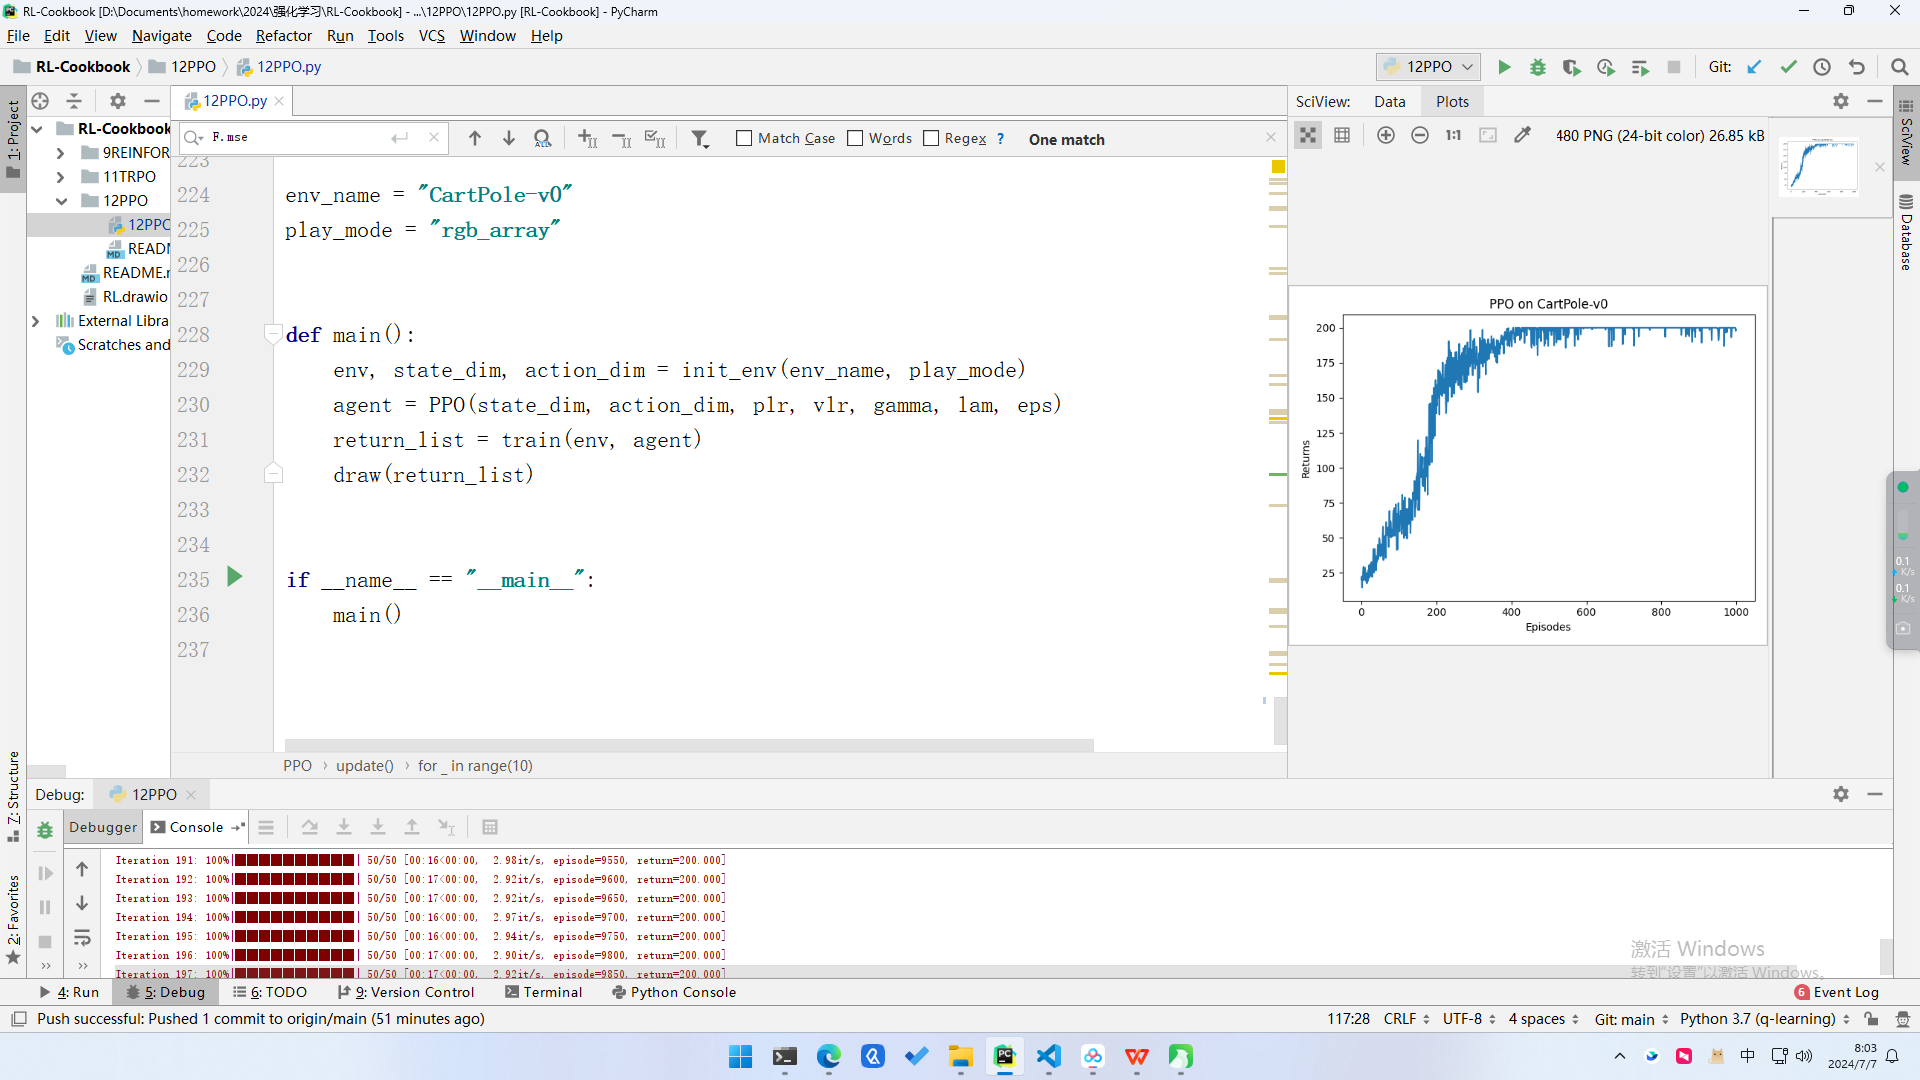
\includegraphics[width=1.2\columnwidth]{image/1.png}
  \caption{带时间的实验结果截图}
\end{figure} 

\par
\begin{figure}[htbp]
  \centering
  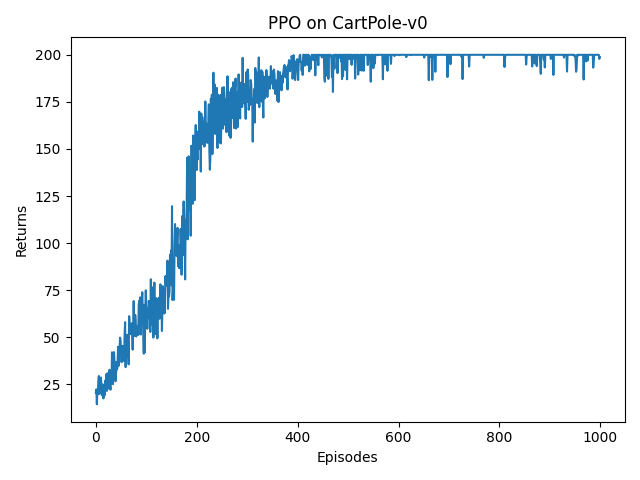
\includegraphics[width=1\columnwidth]{image/2.png}
  \caption{reward随着episodes的变化情况}
  \label{figure-2}
\end{figure} 
根据Figure\ref{figure-2}, 我们发现智能体能够长期达到游戏得分的最高值,即200分。


\section{附录:实验运行环境设置}
请使用python 3.7,进入PPO项目目录执行以下命令:
\begin{lstlisting}
 pip install -r requirements.txt
\end{lstlisting}
安装依赖后运行
\begin{lstlisting}
python PPO.py
\end{lstlisting}




%----------正文----------------------%
\end{document}

